% !TeX root = paper.tex


\chapter{学習データの準備}\label{genri}
%\section{この章で書くこと}
%\begin{itemize}
%	\item djangoの件
%	\item 電車が映っている場面だけ画像で保存
%	\item データセットを作成(識別・分類)
%	\item アノテーションについて
%\end{itemize}

\section{データの収集}
学習データは,車両タイプごとにその車両タイプが映っているYouTubeの動画をダウンロードして,任意の枚数分のランダムなフレームを保存する.その後,保存した画像を識別して電車が映っている画像を保存してレーニングデータとバリデーションデータを収集した.テストデータは様々なウェブサイトから手作業で17種類の各車両の画像を10枚ずつ収集した.
本プロジェクトでは,JR西日本の在来線の電車を識別または分類する.\\
205  207  213  221  223  225  227  271  281  283  285  287  321  323  381  521  683 \\
上記の17種類の画像を集める.
% TODO: \usepackage{graphicx} required

\begin{figure}[htbp]
	\begin{tabular}{cc}
	\begin{minipage}[b]{0.15\linewidth}
			\centering
			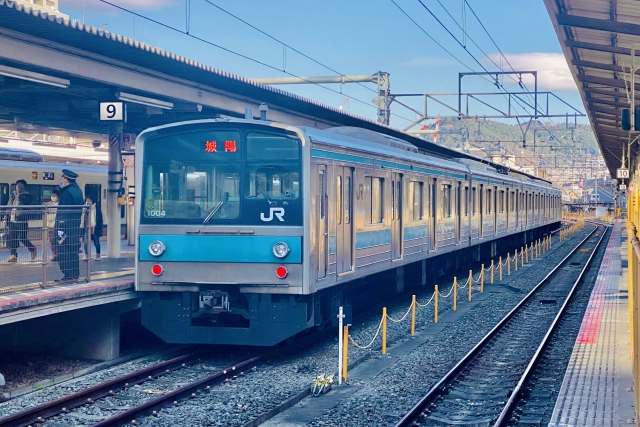
\includegraphics[width=\linewidth]{densya/205.jpg}
			\caption{205系}
			\label{fig:205}
	\end{minipage}
	\begin{minipage}[b]{0.15\textwidth}
		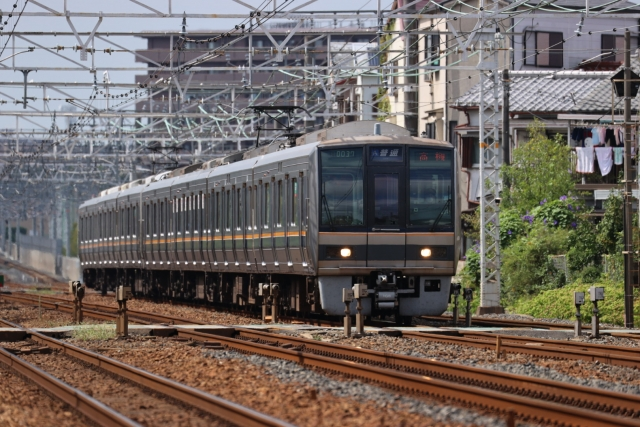
\includegraphics[width=\linewidth]{densya/207.jpg}
		\caption{207系}
		\label{fig:207}
	\end{minipage}
	\begin{minipage}[b]{0.15\textwidth}
		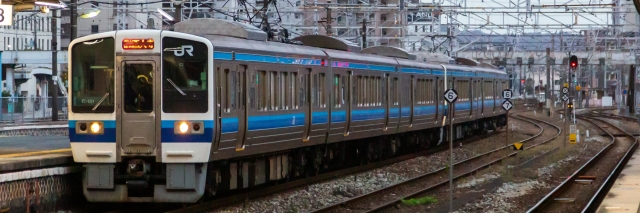
\includegraphics[width=\linewidth]{densya/213.jpg}
		\caption{213系}
		\label{fig:213}
	\end{minipage}
	\begin{minipage}[b]{0.15\textwidth}
		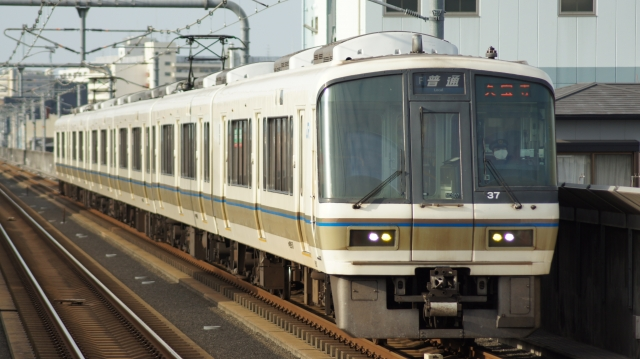
\includegraphics[width=\linewidth]{densya/221.jpg}
		\caption{221系}
		\label{fig:221}
	\end{minipage}
	\begin{minipage}[b]{0.15\textwidth}
		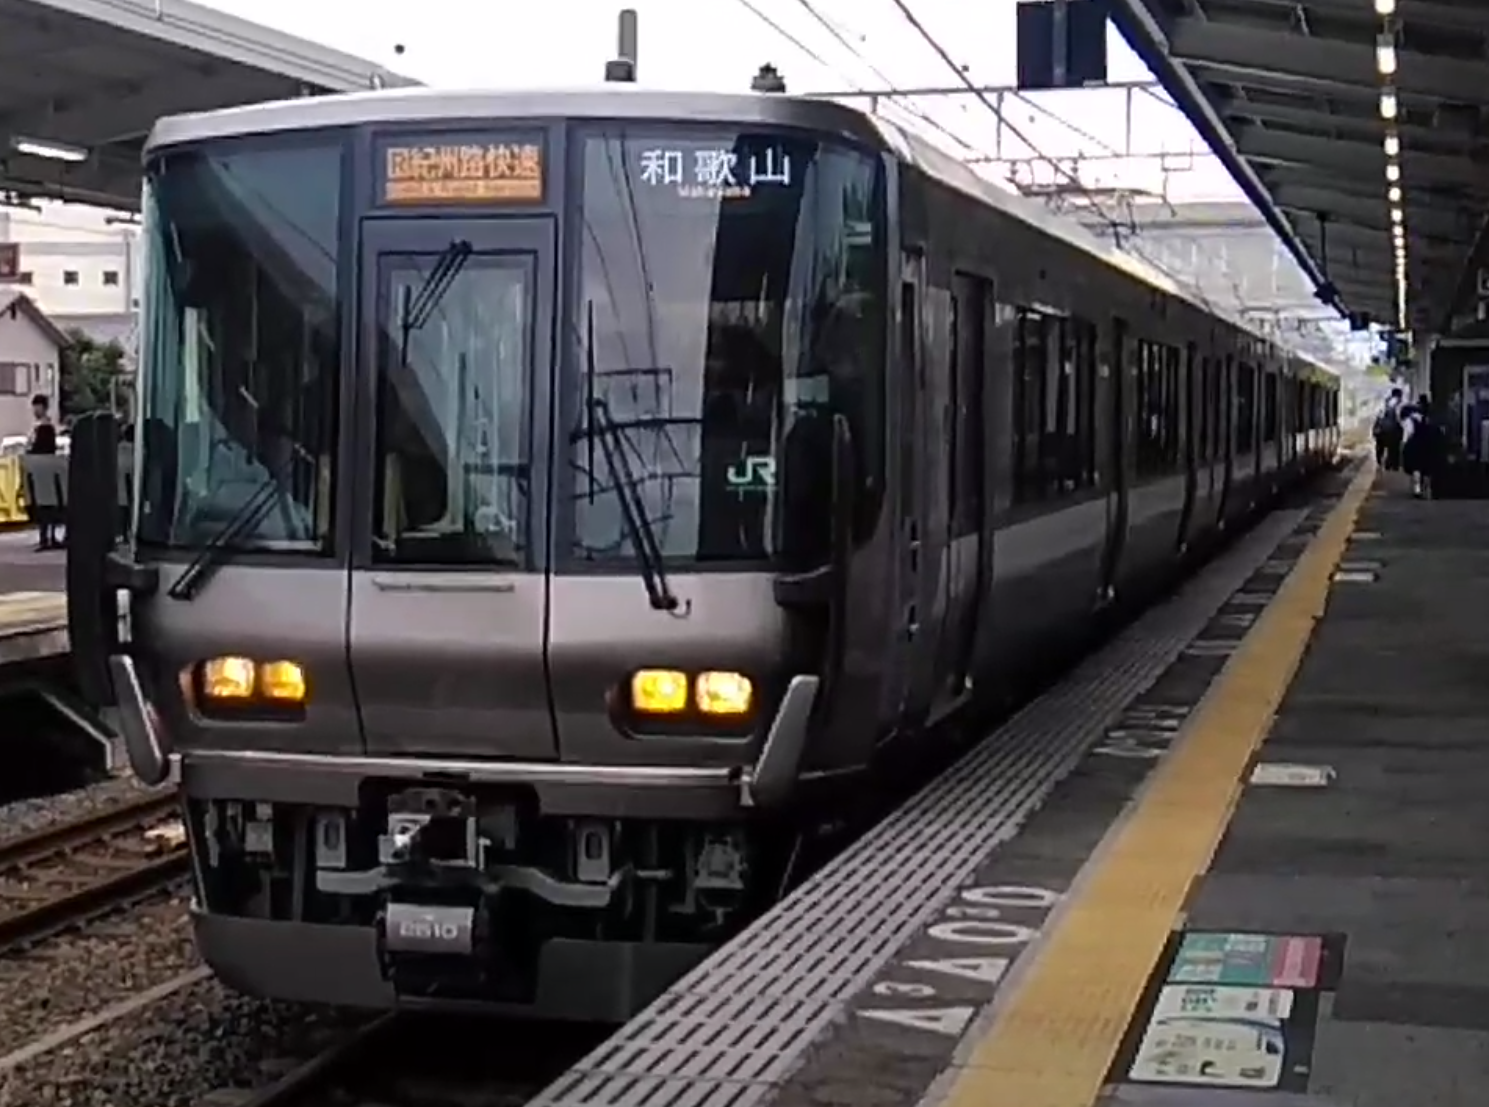
\includegraphics[width=\linewidth]{densya/223.png}
		\caption{223系}
		\label{fig:223}
	\end{minipage}
	\begin{minipage}[b]{0.15\textwidth}
		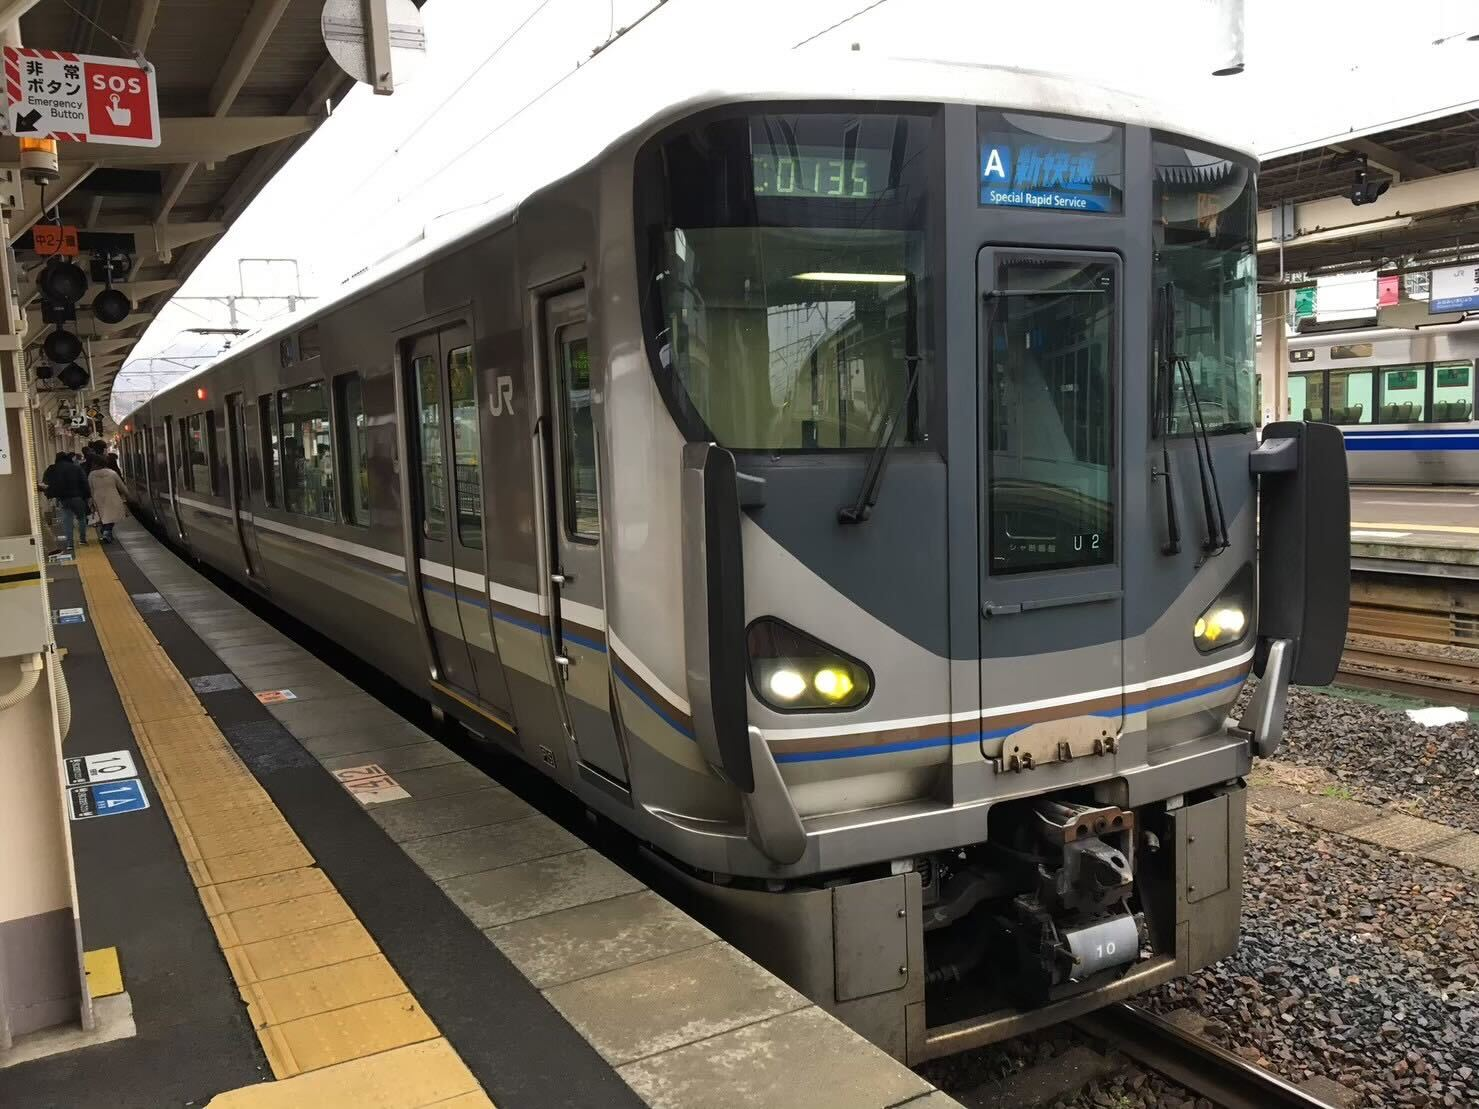
\includegraphics[width=\linewidth]{densya/225.jpg}
		\caption{225}
		\label{fig:225}
	\end{minipage}
	\end{tabular}
\end{figure}

\begin{figure}[htbp]
	\begin{tabular}{cc}
		\begin{minipage}[b]{0.15\linewidth}
			\centering
			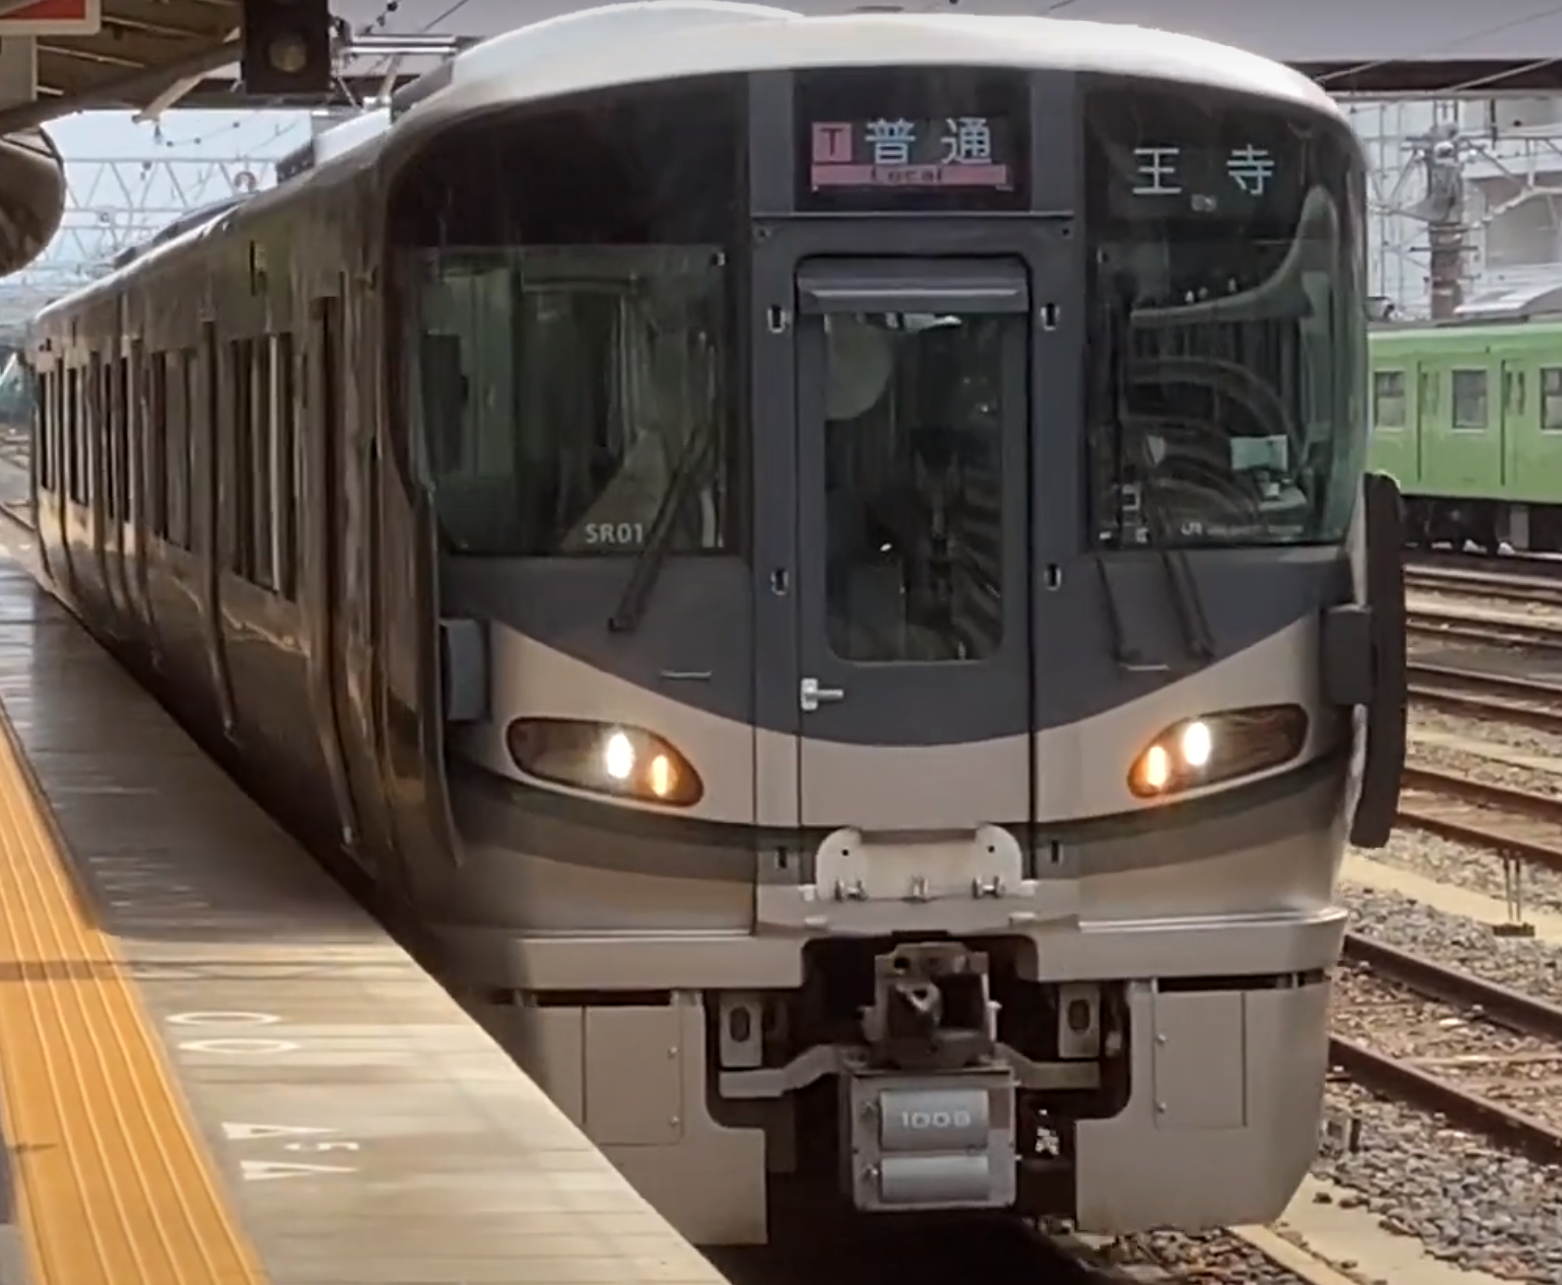
\includegraphics[width=\linewidth]{densya/227.png}
			\caption{227系}
			\label{fig:227}
		\end{minipage}
		\begin{minipage}[b]{0.15\textwidth}
			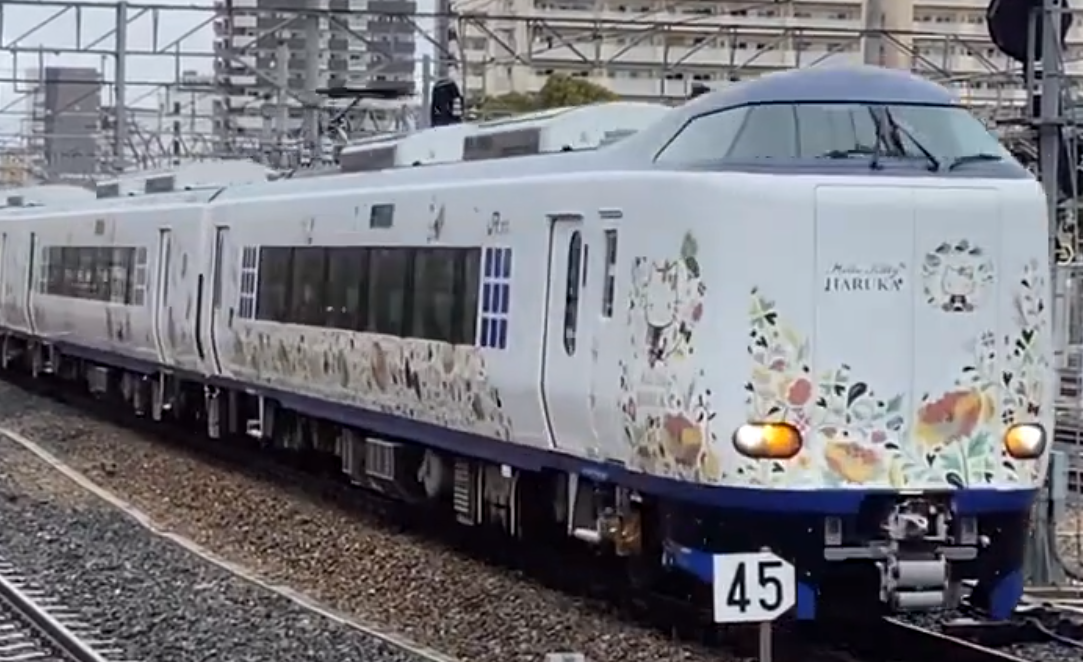
\includegraphics[width=\linewidth]{densya/271.png}
			\caption{271系}
			\label{fig:271}
		\end{minipage}
		\begin{minipage}[b]{0.15\textwidth}
			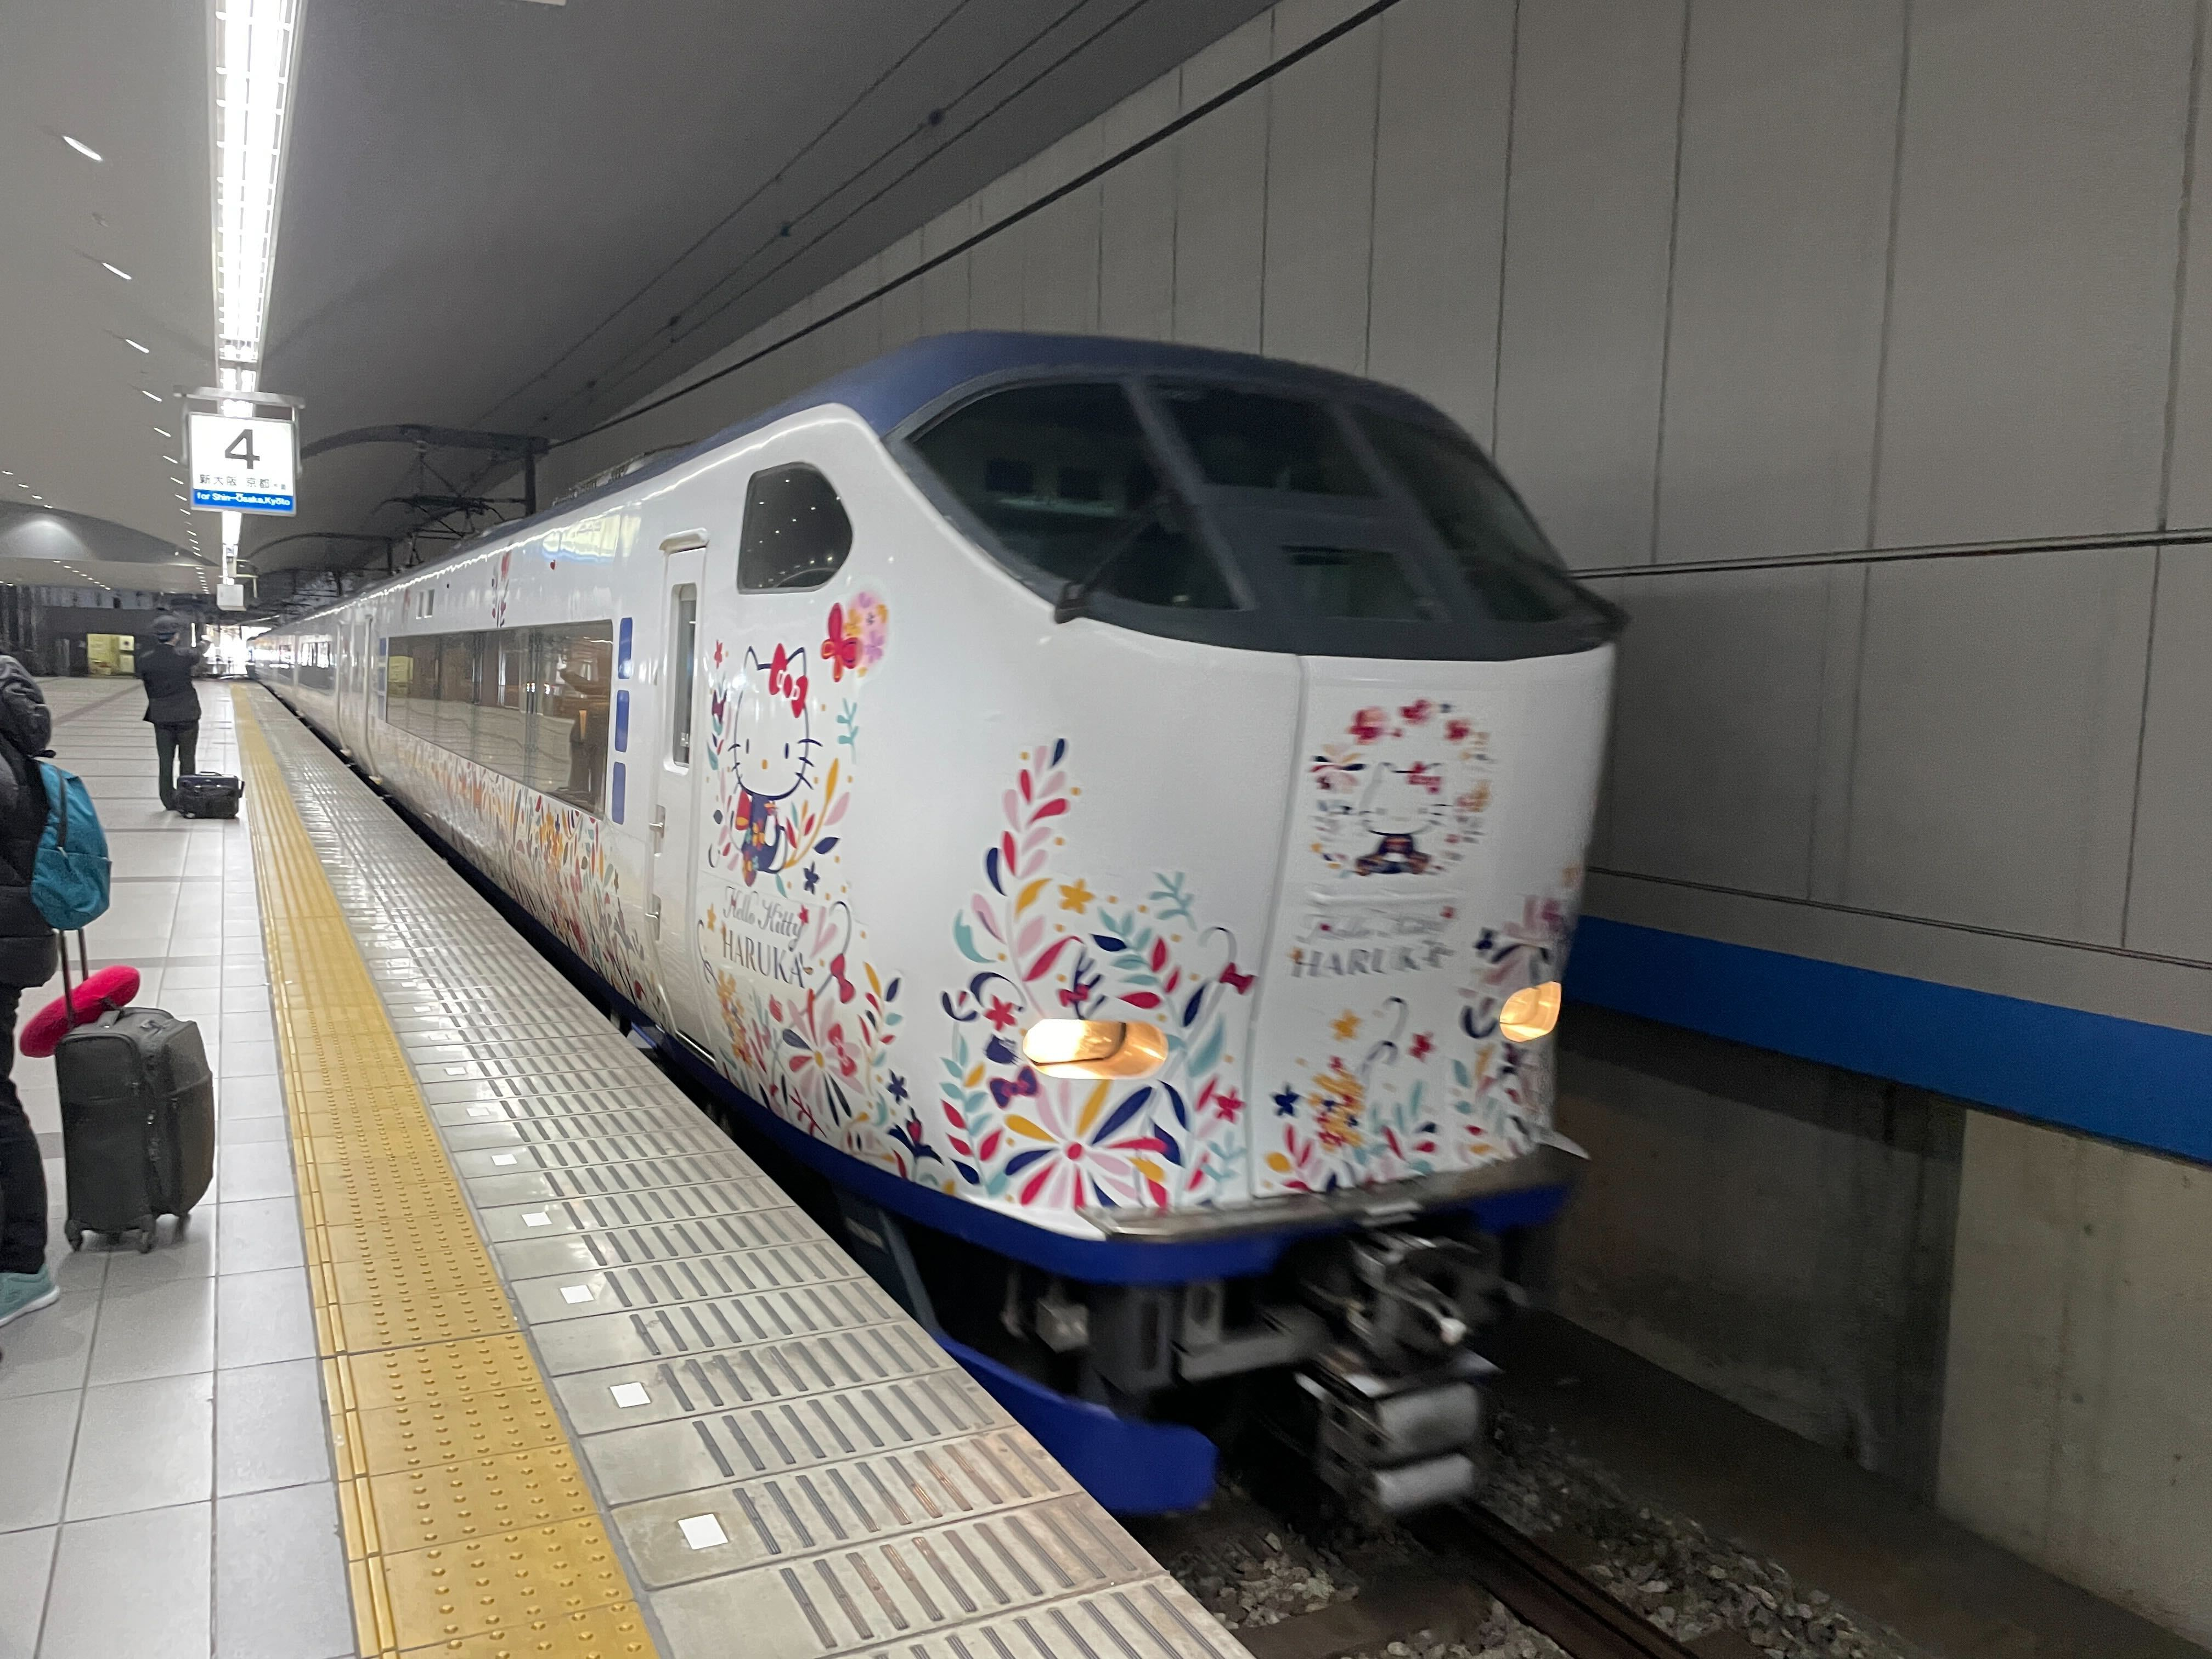
\includegraphics[width=\linewidth]{densya/281.jpg}
			\caption{281系}
			\label{fig:281}
		\end{minipage}
	\begin{minipage}[b]{0.15\textwidth}
		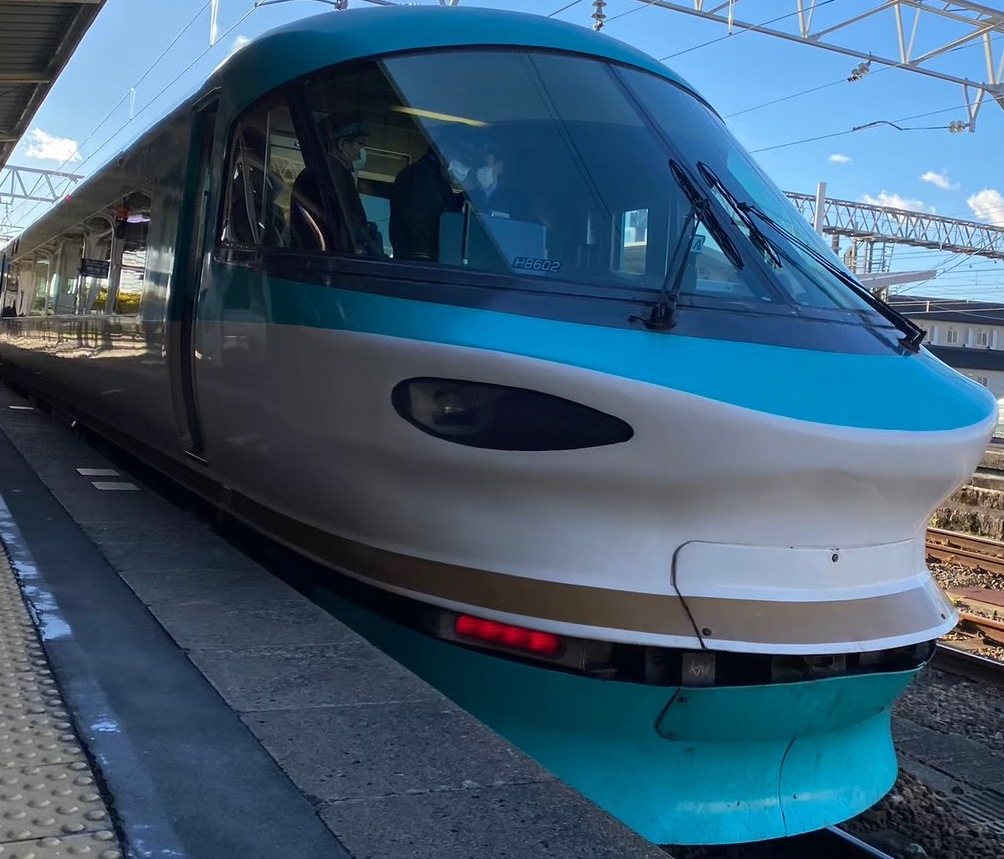
\includegraphics[width=\linewidth]{densya/283.jpg}
		\caption{283系}
		\label{fig:283}
	\end{minipage}
		\begin{minipage}[b]{0.15\textwidth}
			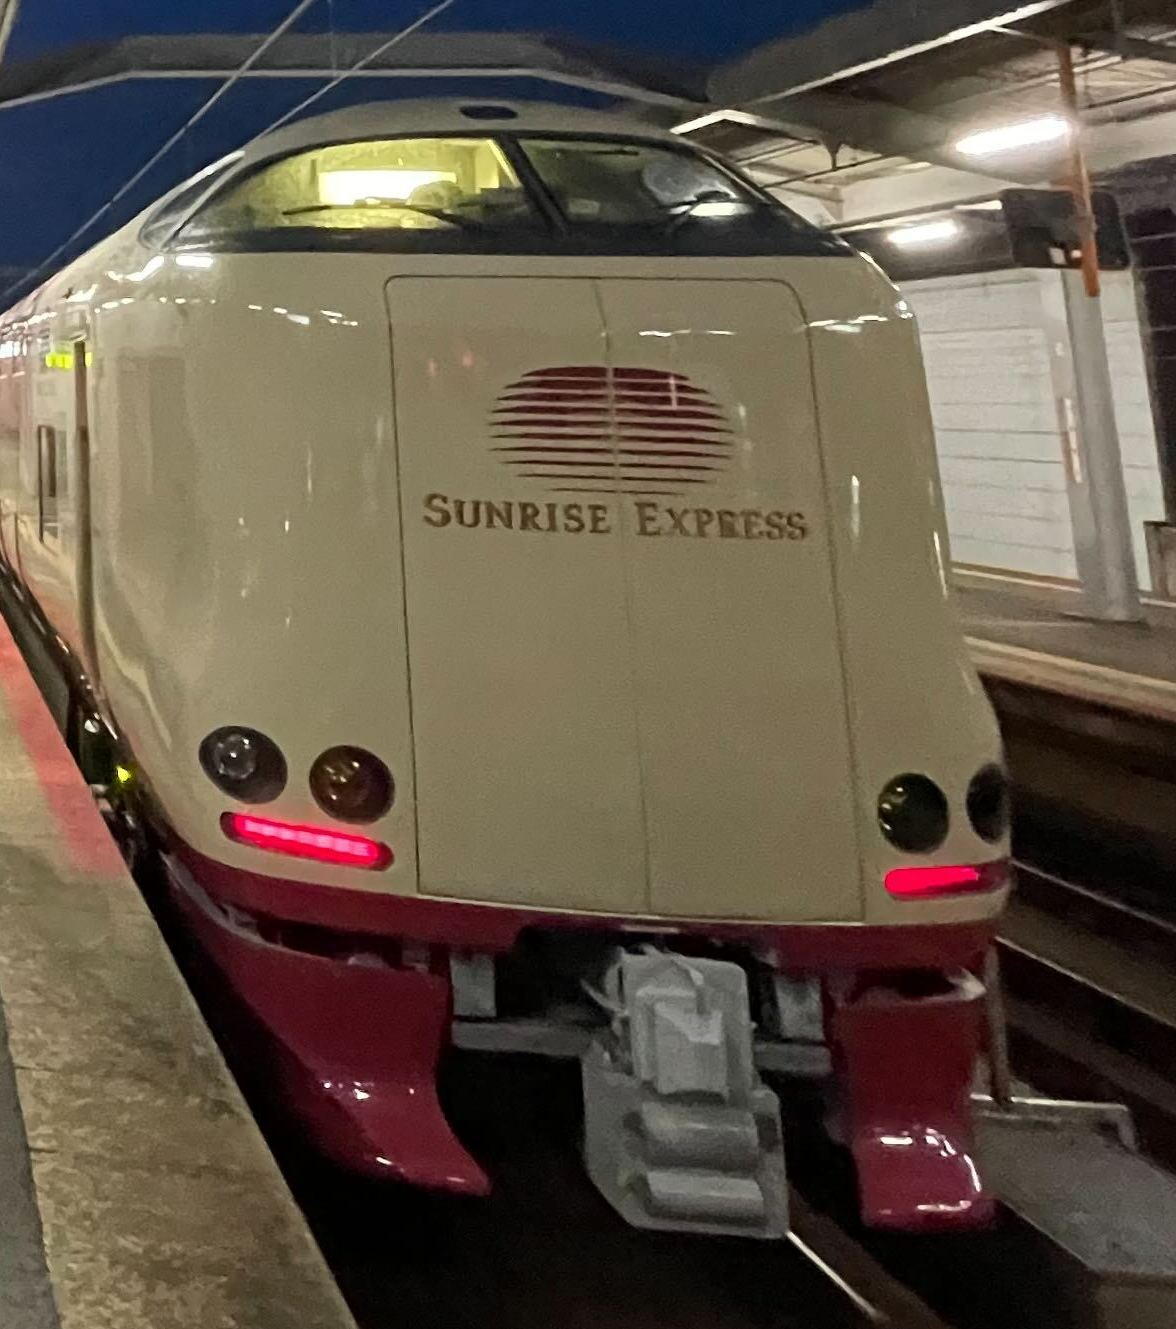
\includegraphics[width=\linewidth]{densya/285.jpg}
			\caption{285系}
			\label{fig:285}
		\end{minipage}
		\begin{minipage}[b]{0.15\textwidth}
			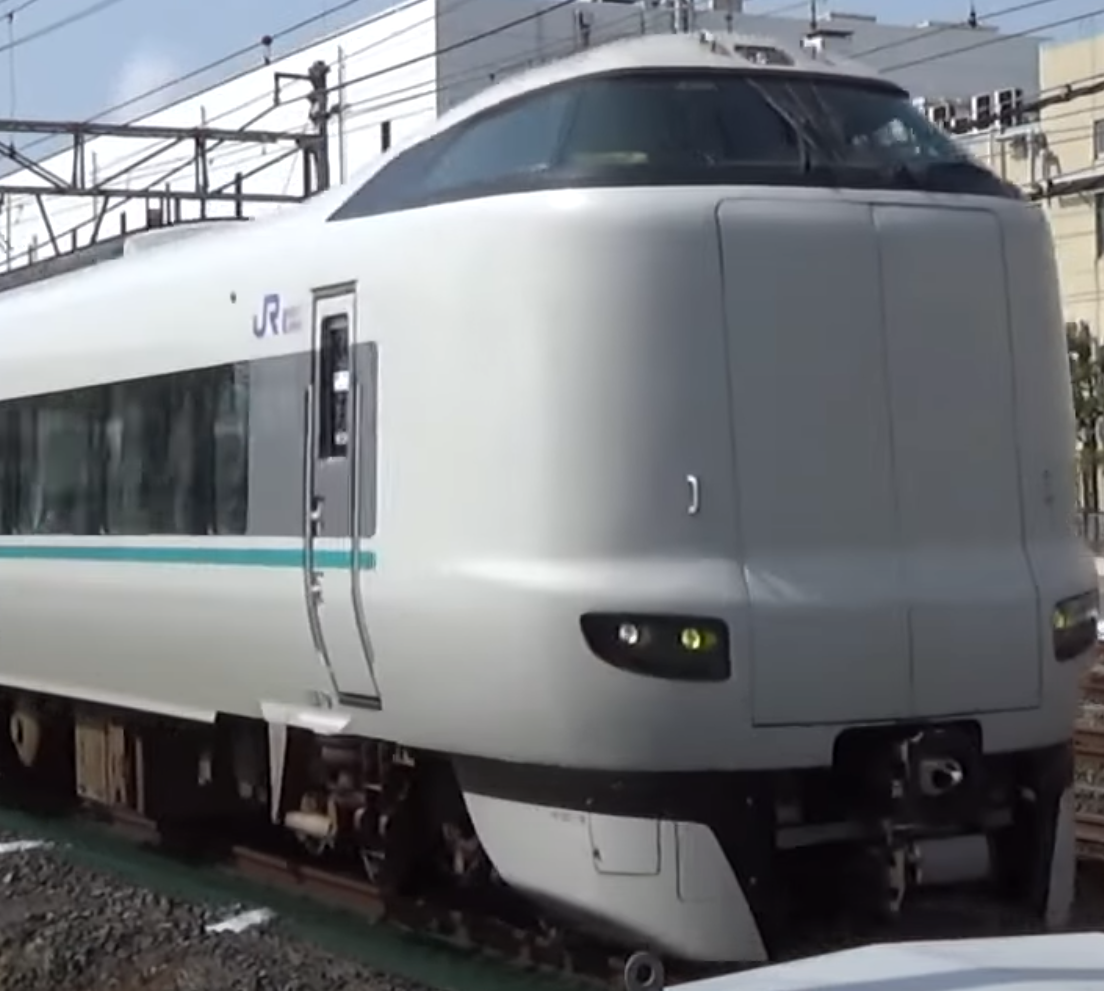
\includegraphics[width=\linewidth]{densya/287.png}
			\caption{287系}
			\label{fig:287}
		\end{minipage}
	
	\end{tabular}
\end{figure}

\begin{figure}[htbp]
	\begin{tabular}{cc}
		\begin{minipage}[b]{0.15\textwidth}
			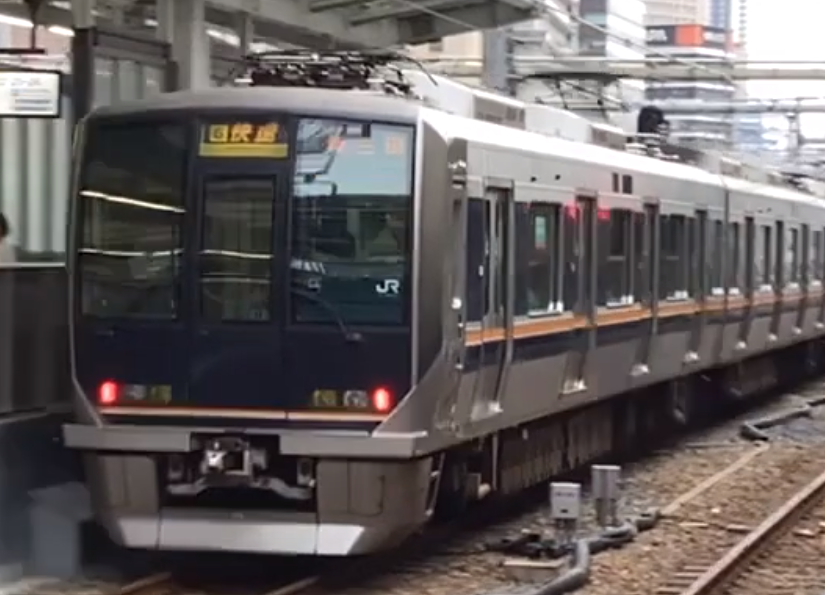
\includegraphics[width=\linewidth]{densya/321.png}
			\caption{321系}
			\label{fig:321}
		\end{minipage}
		\begin{minipage}[b]{0.15\linewidth}
			\centering
			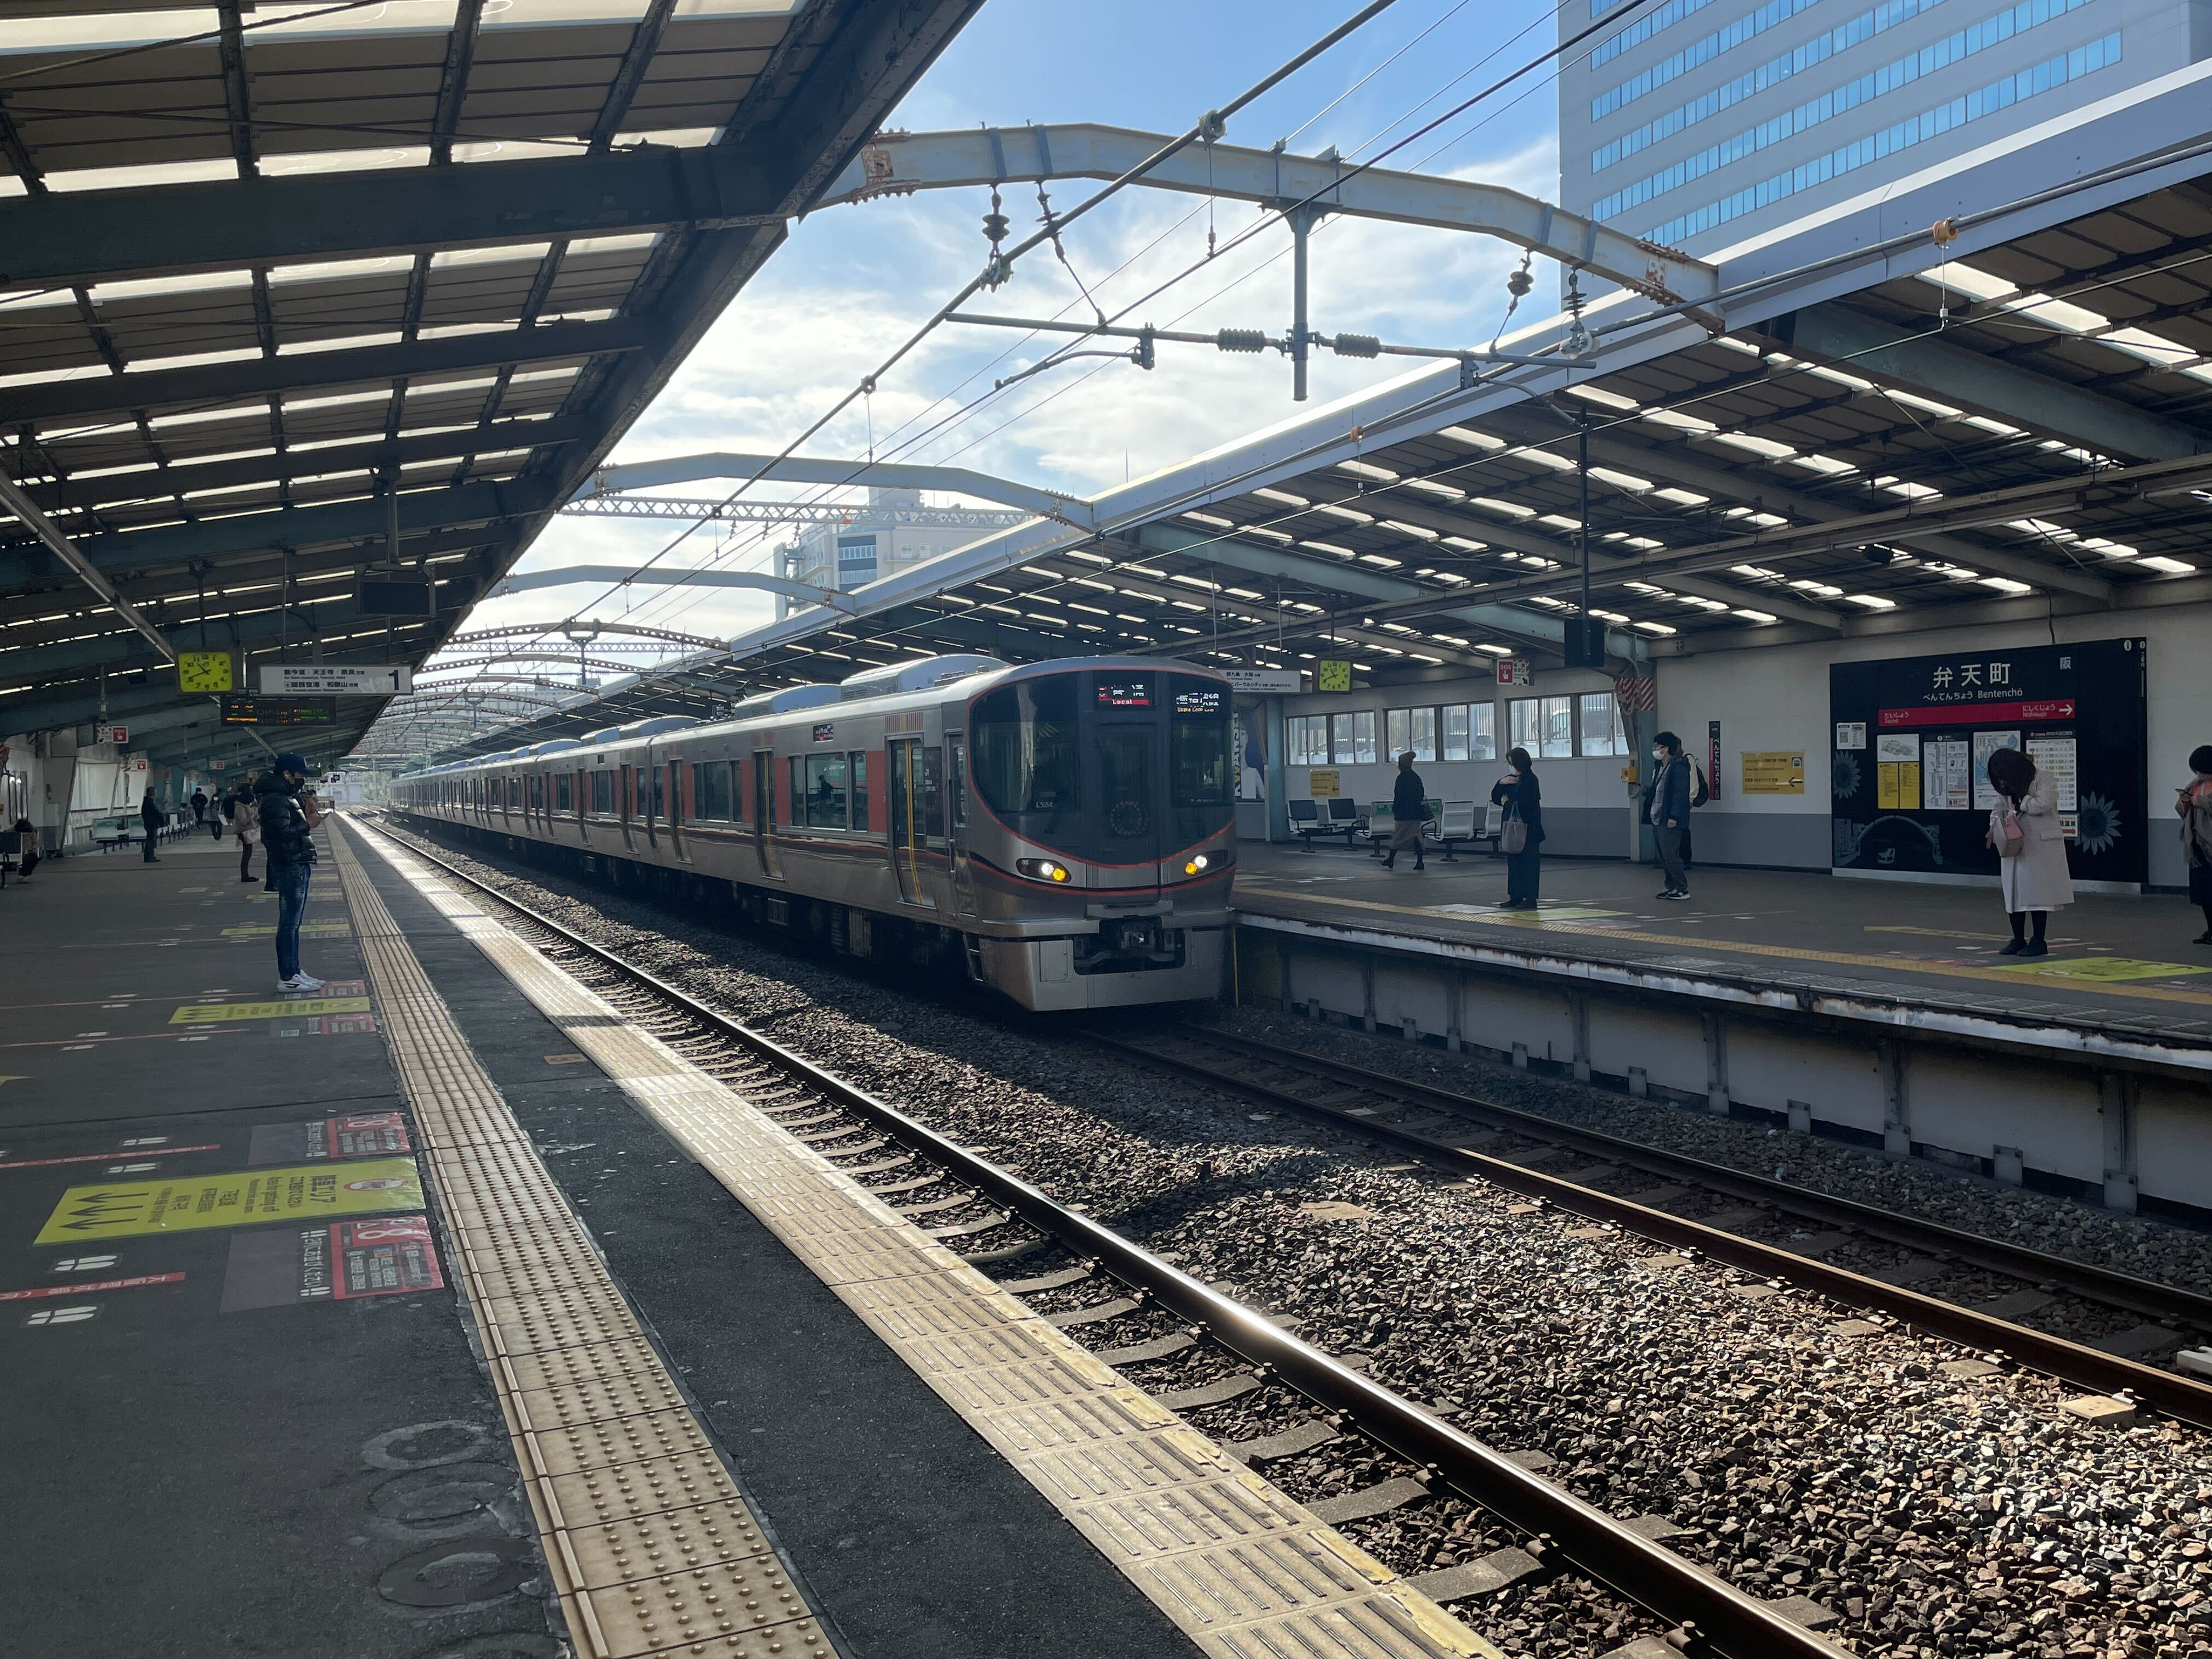
\includegraphics[width=\linewidth]{densya/323.jpg}
			\caption{323系}
			\label{fig:323}
		\end{minipage}
		\begin{minipage}[b]{0.15\textwidth}
			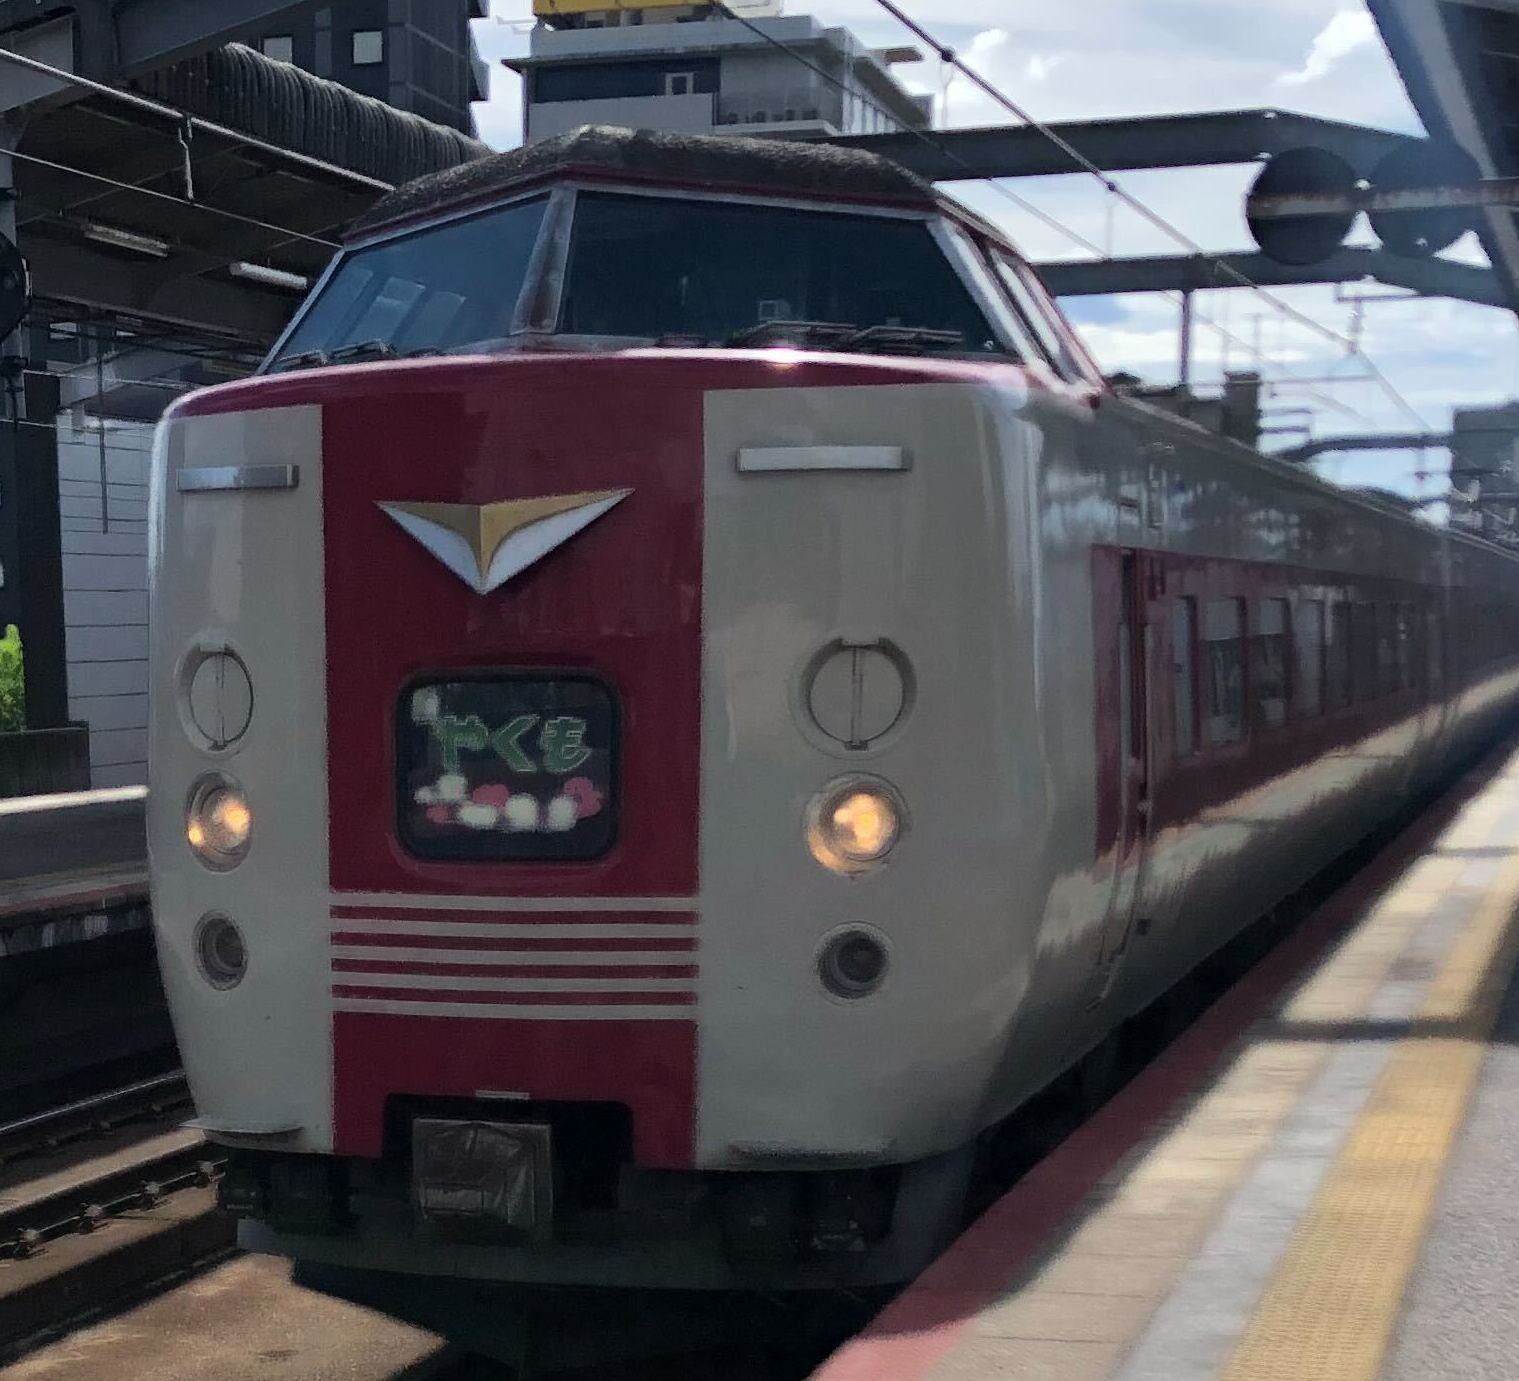
\includegraphics[width=\linewidth]{densya/381.jpg}
			\caption{381系}
			\label{fig:381}
		\end{minipage}
		\begin{minipage}[b]{0.15\textwidth}
			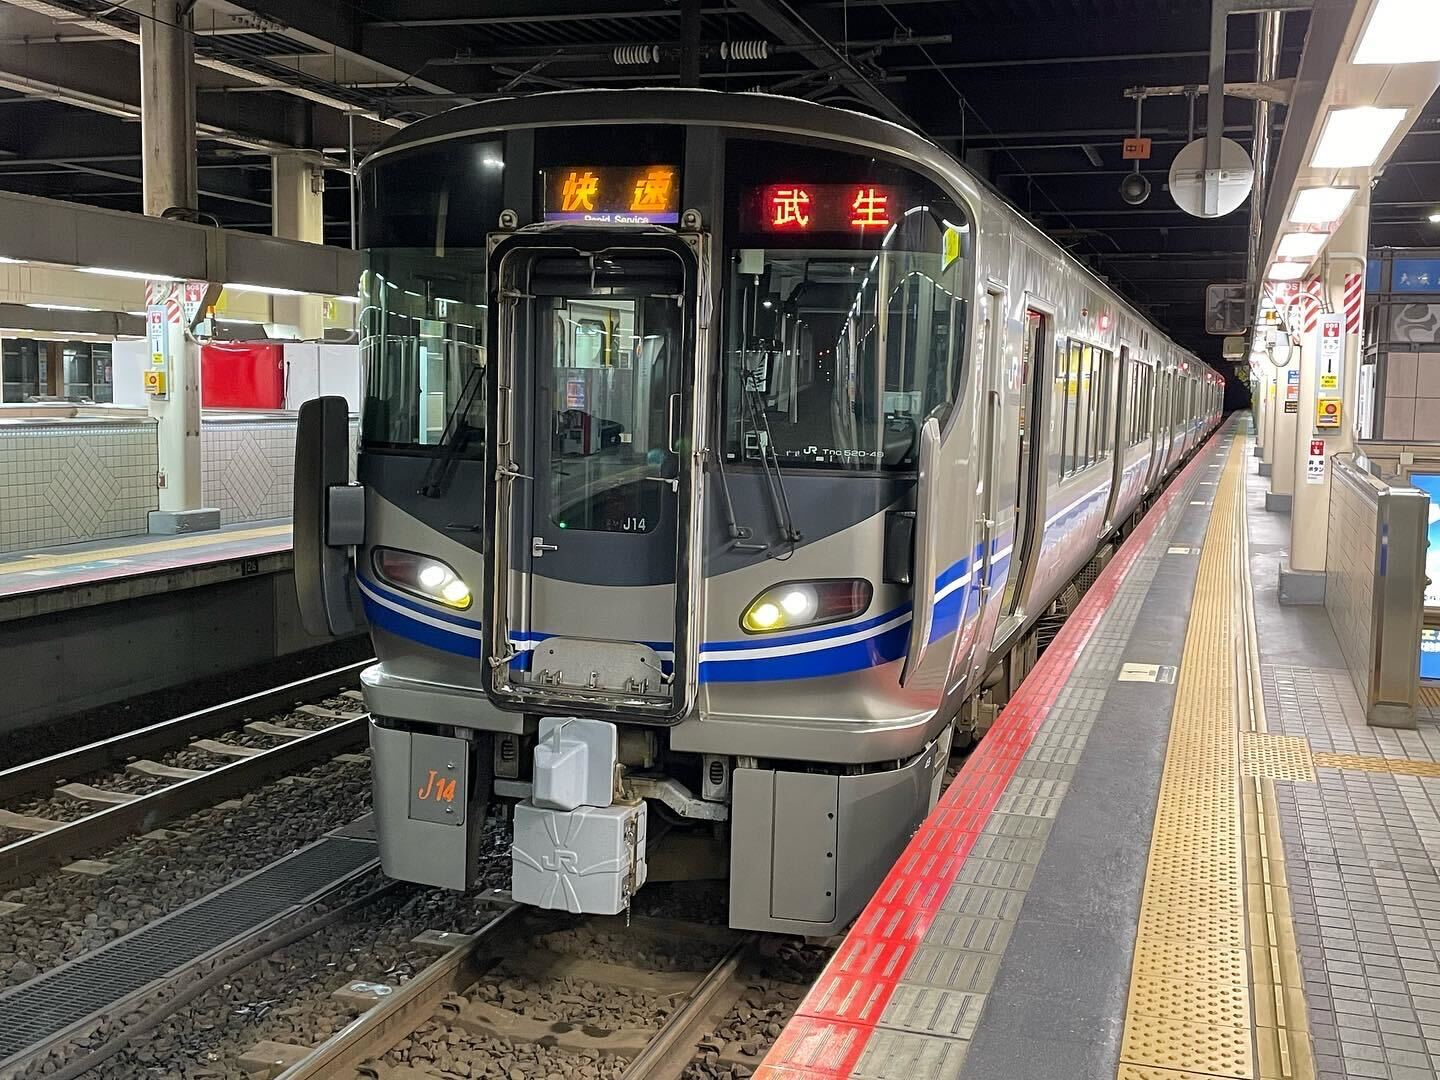
\includegraphics[width=\linewidth]{densya/521.jpg}
			\caption{521系}
			\label{fig:521}
		\end{minipage}
		\begin{minipage}[b]{0.15\textwidth}
			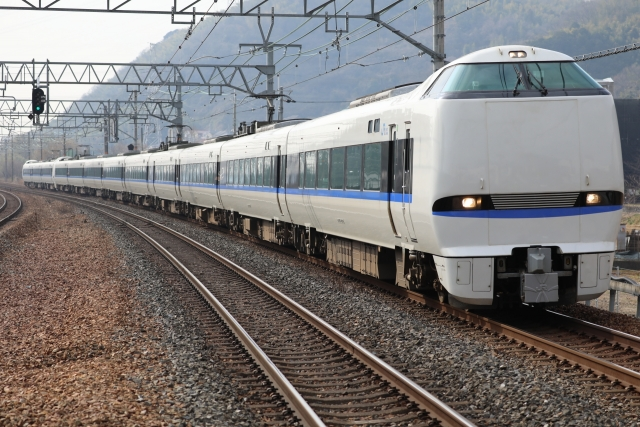
\includegraphics[width=\linewidth]{densya/683.jpg}
			\caption{683系}
			\label{fig:683}
		\end{minipage}
	\end{tabular}
\end{figure}


\subsection{動画の連結と保存}
動画の保存にはyt-dlpという動画や音声をダウンロードするプログラムを使う.
1〜3種類の動画の任意の秒数をダウンロードしてそれぞれの動画を連結して一つの動画にするwebアプリケーションをPythonのフレームワークの一つであるDjangoを使って作成した.
%	\red{画像は後で変える,大きさを揃える}\\
	作成したwebアプリケーションは,図\ref{test3}のようになっている.
	YouTube上の動画のURLと開始時刻(秒),終了時刻(秒),車両タイプ名を入力して,1〜3種類の動画を保存し連結して一つの動画にしている.
	
\begin{figure}[H]
	\includegraphics [width=0.9\linewidth]{chap3/fig/test3.png}
	\caption{動画のダウンロード3,あとで画像を差し替え}
	\label{test3}
\end{figure}

\subsection{画像の保存}
保存した動画を利用して指定した枚数分のランダムなフレームを保存する.保存した画像を識別し電車が映っている画像だけを保存す,トレーニングデータとバリデーションデータを収集した.
テストデータは様々なウェブサイトから手作業で17種類の各車両の画像を10枚ずつ収集した.
車両タイプごとに保存した画像の枚数を図\ref{fig:chart}に示す.

% TODO: \usepackage{graphicx} required

% TODO: \usepackage{graphicx} required
\begin{figure}[H]
	\centering
	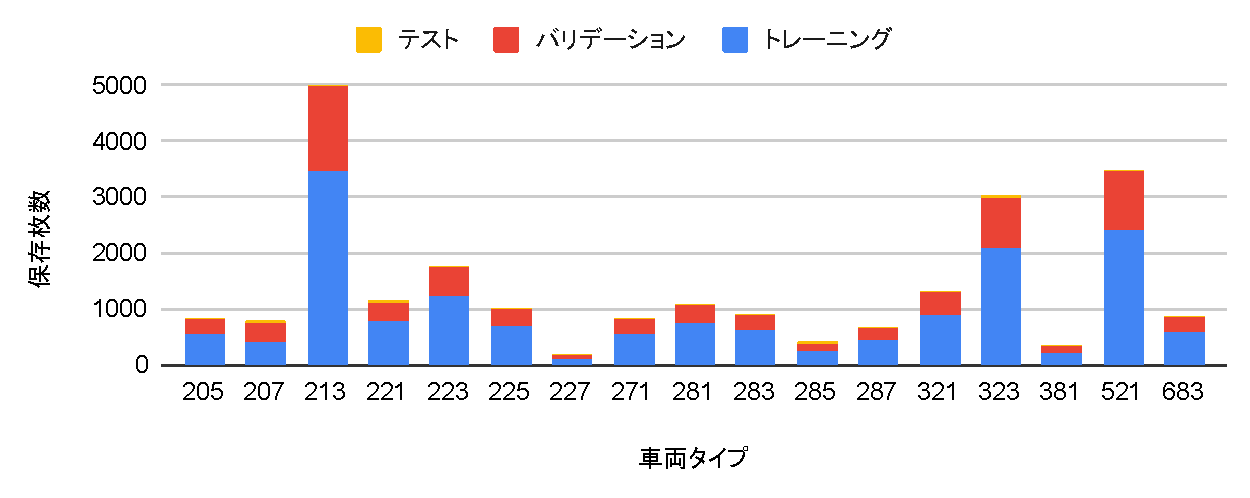
\includegraphics[width=\linewidth]{chap3/fig/chart2}
	\caption{各車両タイプ(全17種)の保存枚数}
	\label{fig:chart}
\end{figure}



\section{データセットの作成}
%\subsection{データセットの構造}

識別モデル用データセットと分類モデル用データセットの学習時に使用する画像は同じものを使う.識別モデル用のデータセットには画像のアノテーション情報が必要なので,アノテーションも行った.
このテストデータセットと作成したモデルを使って分類または識別を行い,モデルの性能の評価を行う.
%\subsection{アノテーション}
%https://www.dir.co.jp/world/entry/solution/annotation
アノテーションとは、機械学習の分類の一つである教師あり学習において,分析対象データにラベルを付与するプロセスである.画像にバウンディングボックスと呼ばれる四角形を描画しクラス番号を指定する.バウンディングボックスを描画することでその画像に写っている物体の座標情報を取得することができる.クラス番号とは,判別したいものリストを作成し,画像に写っている物体に対応した,リストのインデックスのことである.アノテーションをした結果は,識別モデルの学習時に使用する.

一般的にアノテーションは,手作業で行うものである.
しかし,数千枚の画像を手作業で行うことは難しいので,自動で行えるようにした.
分類モデル用のデータセットでは一枚の画像に電車が一つだけ映っている.その画像を配布されている識別用モデルで識別することでクラス番号と電車が映っている座標情報をテキストに書き込む.その後,本プロジェクトで識別する車両タイプリストに対応するクラス番号を上書きすることで,分類モデル用のデータセットから識別モデル用のデータセットを作成した.

